\documentclass[urlcolor=blue,dvipsnames]{beamer}

\usepackage[utf8]{inputenc}
\usepackage{fancybox,fancyvrb}
\usepackage{environ,xspace,empheq}
\usepackage{tikz}
\hypersetup{colorlinks,linkcolor=,urlcolor=cyan}

\beamertemplatenavigationsymbolsempty
\setbeamertemplate{footline}[frame number]
\usetheme{Pittsburgh}

\newcommand\enumnum[1]{{\renewcommand{\insertenumlabel}{#1}%
      \usebeamertemplate{enumerate item} \,}}

\newcommand{\grad}{\nabla}
\newcommand{\ih}{\boldsymbol{\hat{\textbf{\i}}}}
\newcommand{\jh}{\boldsymbol{\hat{\textbf{\j}}}}
\newcommand{\vF}{\boldsymbol{\vec{\textbf{F}}}}
\newcommand{\Matlab}{\textsc{Matlab}\xspace}
\newcommand{\Octave}{\textsc{Octave}\xspace}


\title{9.2 Runge-Kutta methods}

\subtitle{a lesson for MATH F302 Differential Equations}

\author{Ed Bueler, Dept.~of Mathematics and Statistics, UAF}

\date{\tiny \today}


\begin{document}
\setbeamertemplate{itemize item}{$\bullet$}
\setbeamertemplate{itemize subitem}{$\circ$}
\renewcommand{\thefootnote}{{\color{green} \arabic{footnote}}}

\begin{frame}
\titlepage

\centerline{\tiny for textbook: \, D. Zill, \emph{A First Course in Differential Equations with Modeling Applications}, 11th ed.}
%\color{green!40!blue}
\end{frame}


\begin{frame}{the Runge-Kutta happy family}

\begin{itemize}
\item these slides describe and test the most-famous \emph{Runge-Kutta} (RK) method, namely \alert{(classical) RK4} which is \alert{order 4}
    \begin{itemize}
    \item RK4 dates to $\sim$1900, \emph{before} invention of electronic computers
    \item there are dozens of useful RK methods of all orders $\ge 1$
    \item Euler's method is the order 1 RK method
    \item improved Euler is an order 2 RK method
    \item $\infty$ly-many methods in the family \dots
    \end{itemize}
\item RK4 was accurate enough for most ODE solutions in science and engineering until $\sim$1960
\item better computers and programming languages allow reliable/debugged implementations of better-than-RK4 methods like \texttt{ode45} in \Matlab/\Octave
    \begin{itemize}
    \item \dots which are \emph{not} a lot more accurate
    \item instead, modern methods like \texttt{ode45} are \emph{adaptive} so the user does not need to choose a step size $h$
    \end{itemize}
\end{itemize}
\end{frame}


\begin{frame}{improved Euler dance}

\begin{itemize}
\item ODE IVP: $\frac{dy}{dt} = t-y^2$, $y(0)=1$
\item show on the direction field: improved Euler with $h=1$
\end{itemize}

\hfill 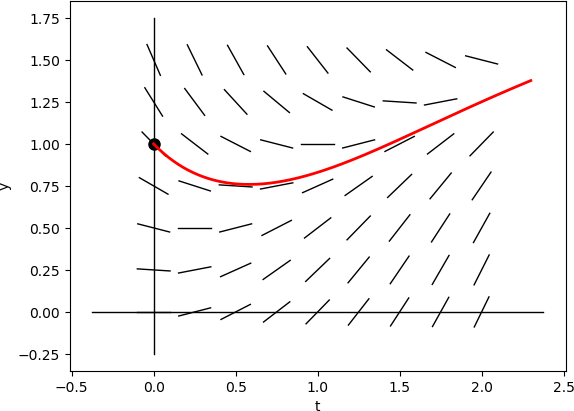
\includegraphics[width=0.8\textwidth]{figs/for-rk4-dir-field}
\end{frame}


\begin{frame}{RK4 dance}

\begin{itemize}
\item ODE IVP: $\frac{dy}{dt} = t-y^2$, $y(0)=1$
\item show on the direction field: RK4 with $h=1$
\end{itemize}

\hfill 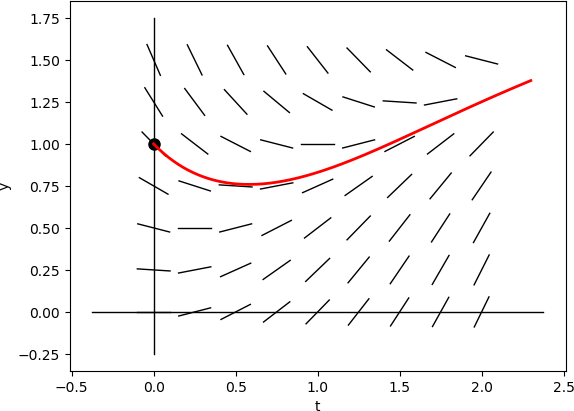
\includegraphics[width=0.8\textwidth]{figs/for-rk4-dir-field}
\end{frame}


\begin{frame}{RK4 \alert{precise} dance}

\begin{itemize}
\item ODE IVP: $\frac{dy}{dt} = t-y^2$, $y(0)=1$
\item show on the direction field: RK4 with $h=1$
\end{itemize}

\hfill 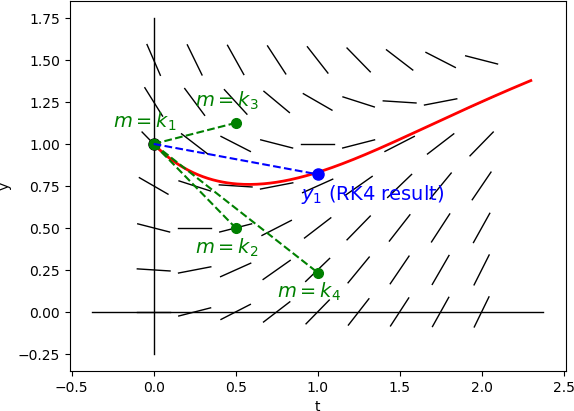
\includegraphics[width=0.8\textwidth]{figs/result-rk4-dir-field}
\end{frame}


\begin{frame}{the RK4 formulas}

\small
\begin{itemize}
\item usually written using four slopes ``$k_i$'' from direction field
\item update the $y$-value by a weighted average of these slopes:

\vspace{-6mm}
\begin{minipage}[t]{0.4\textwidth}
\begin{align*}
k_1 &= f(t_n,y_n) \\
k_2 &= f(t_n+\frac{h}{2},y_n+\frac{h}{2} k_1) \\
k_3 &= f(t_n+\frac{h}{2},y_n+\frac{h}{2} k_2) \\
k_4 &= f(t_n+h,y_n+h k_3)
\end{align*}
\end{minipage}\begin{minipage}[t]{0.45\textwidth}
\vspace{10mm}

$$\implies y_{n+1} = y_n + h\, \frac{k_1 + 2 k_2 + 2 k_3 + k_4}{6}$$
\end{minipage}
\item here are the formulas for improved Euler, written the same way:

\vspace{-6mm}
\begin{minipage}[t]{0.4\textwidth}
\begin{align*}
k_1 &= f(t_n,y_n) \\
k_2 &= f(t_n+h,y_n+h k_1)
\end{align*}
\end{minipage}
\begin{minipage}[t]{0.4\textwidth}
\vspace{2mm}

$$\implies y_{n+1} = y_n + h\, \frac{k_1 + k_2}{2}$$
\end{minipage}
\item here is Euler itself, written the same way:
$$k_1 = f(t_n,y_n) \qquad \implies y_{n+1} = y_n + h\, k_1$$
\end{itemize}
\end{frame}


\begin{frame}{RK4 scheme in one diagram}

\begin{columns}
\begin{column}{0.35\textwidth}
\small
\begin{itemize}
\item drawing this sketch, or similar, will be an extra credit problem on Midterm 2
\end{itemize}
\end{column}
\begin{column}{0.65\textwidth}
\hfill 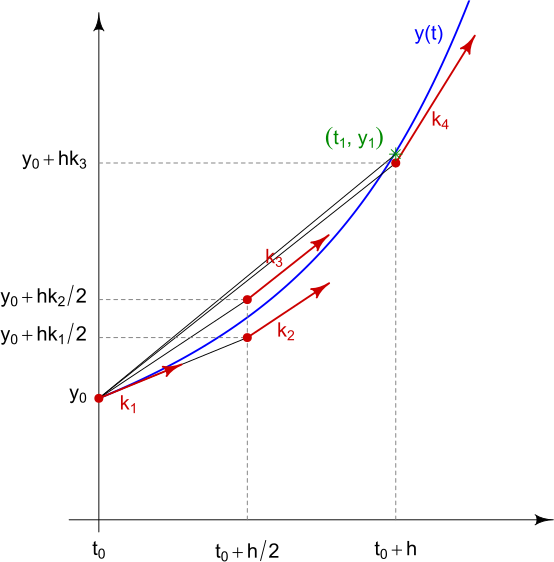
\includegraphics[width=\textwidth]{figs/rk4diagram}
\end{column}
\end{columns}
\end{frame}


\begin{frame}{exercise \#7 in \S9.2}

\begin{itemize}
\item FIXME
\end{itemize}
\end{frame}


\begin{frame}{exercise \#7 in \S9.2, cont.}

\begin{itemize}
\item x
\end{itemize}
\end{frame}


\begin{frame}[fragile]
\frametitle{there are \emph{bad} ODE IVPs out there!}

\begin{itemize}
\item inspired by exercise \#15 in \S9.2
\item \emph{exercise.}  for this ODE IVP, find $y(1.4)$:
    $$y' = x^2 + y^3, \quad y(1)=1,$$
\end{itemize}

\hfill 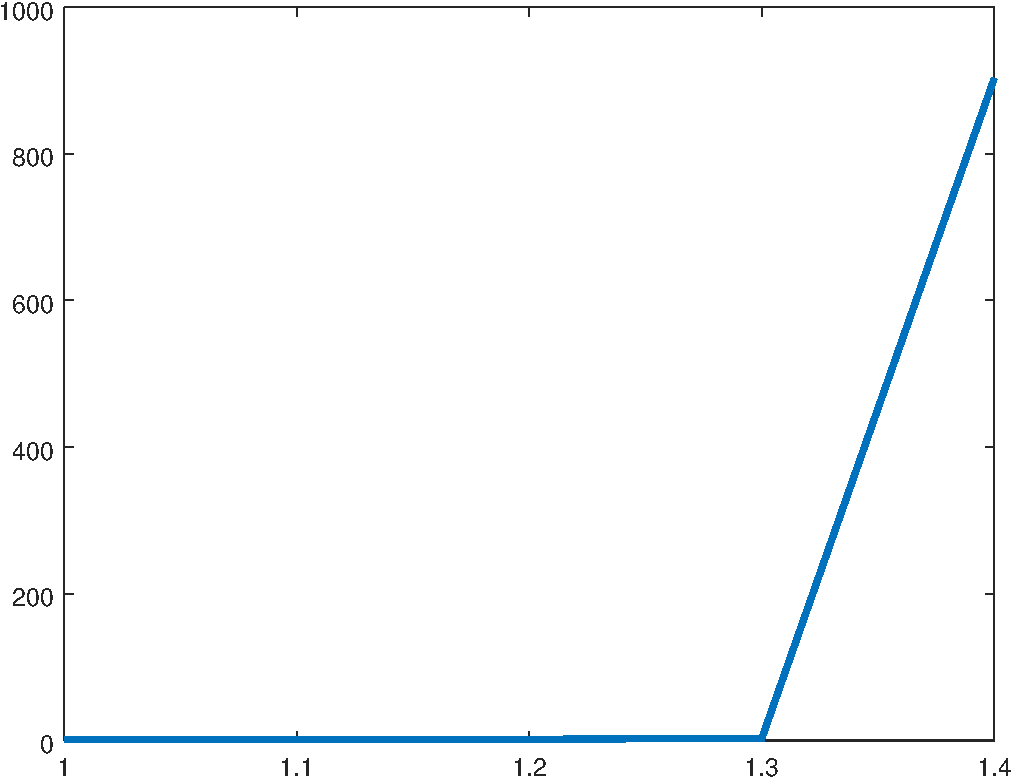
\includegraphics[width=0.3\textwidth]{figs/blowuprk4}

\vspace{-20mm}
\noindent \emph{solution.}
\begin{Verbatim}[fontsize=\footnotesize]
>> f = @(x,y) x^2 + y^3;
>> [xx,yy] = rk4(f,[1,1.4],0.1);
>> plot(xx,yy)
>> yy
yy =
      1      1.2511      1.6934      2.9425      903.03
>> [xxx,yyy] = ode45(f,[1,1.4],1);
warning:  Solving was not successful.  The iterative integration
loop exited at time t = 1.355695 before the endpoint at
tend = 1.400000 was reached.  This may happen if the stepsize
becomes too small.  Try to reduce the value of 'InitialStep'
and/or 'MaxStep' with the command 'odeset'.
warning: called from ...
\end{Verbatim}

\end{frame}


\begin{frame}[fragile]
\frametitle{when does it blow up?}

\begin{itemize}
\item for this ODE IVP, find $y(1.4)$:\footnote{``find $y(1.4)$'' \emph{is} a trick question \dots never gets that far!} \quad $y' = x^2 + y^3, \quad y(1)=1$
\end{itemize}

\begin{Verbatim}[fontsize=\footnotesize]
>> [xxx,yyy] = ode45(f,1:0.00001:1.35569,1);
>> plot(xxx,yyy)                               <-- PLOT BELOW
>> [xxx,yyy] = ode45(f,1:0.00001:1.35570,1);   <-- GENERATES WARNING
\end{Verbatim}

\hfill 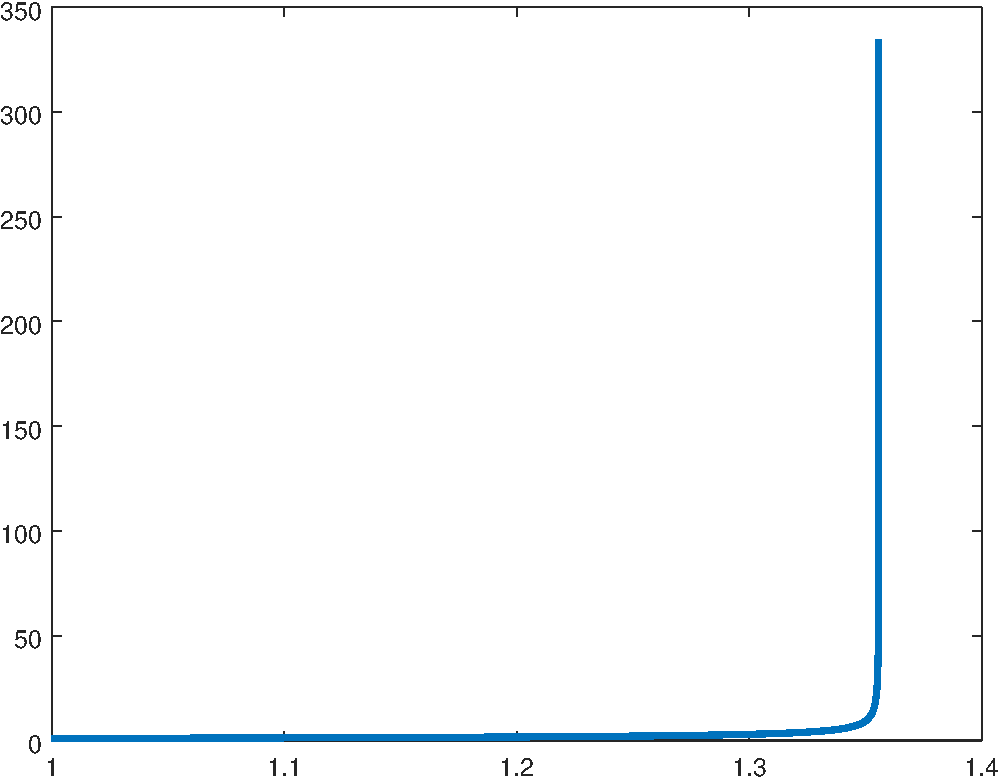
\includegraphics[width=0.55\textwidth]{figs/blowupode45}
\end{frame}


\begin{frame}{RK4 and \texttt{ode45} summary}

\begin{itemize}
\item the last example shows one reason nonlinear ODEs are interesting \dots the \emph{problems} can be badly behaved
\item but RK4 is the first of powerful tools to handle the problems via highly-accurate numerical approximations
\item the black-box \texttt{ode45} is a combination of an ``RK4'' and an ``RK5'' that allows adaptive step size computations
   \begin{itemize}
   \item the RK4 and RK5 formulas use the same intermediate locations to get slopes from the direction field
   \item if you really want to know, see FIXME
   \end{itemize}
\end{itemize}
\end{frame}


\begin{frame}{expectations}

\begin{itemize}
\item just watching this video is \emph{not} enough!
     \begin{itemize}
     \item see ``found online'' videos and stuff at

     \centerline{\href{https://bueler.github.io/math302/week10.html}{\tt \color{cyan} bueler.github.io/math302/week10.html}}
     \item \emph{read} section 9.2 in the textbook
     \item \emph{do} the WebAssign exercises for section 9.2
     \end{itemize}
\end{itemize}
\end{frame}

\end{document}

